\documentclass[1p]{elsarticle_modified}
%\bibliographystyle{elsarticle-num}

%\usepackage[colorlinks]{hyperref}
%\usepackage{abbrmath_seonhwa} %\Abb, \Ascr, \Acal ,\Abf, \Afrak
\usepackage{amsfonts}
\usepackage{amssymb}
\usepackage{amsmath}
\usepackage{amsthm}
\usepackage{scalefnt}
\usepackage{amsbsy}
\usepackage{kotex}
\usepackage{caption}
\usepackage{subfig}
\usepackage{color}
\usepackage{graphicx}
\usepackage{xcolor} %% white, black, red, green, blue, cyan, magenta, yellow
\usepackage{float}
\usepackage{setspace}
\usepackage{hyperref}

\usepackage{tikz}
\usetikzlibrary{arrows}

\usepackage{multirow}
\usepackage{array} % fixed length table
\usepackage{hhline}

%%%%%%%%%%%%%%%%%%%%%
\makeatletter
\renewcommand*\env@matrix[1][\arraystretch]{%
	\edef\arraystretch{#1}%
	\hskip -\arraycolsep
	\let\@ifnextchar\new@ifnextchar
	\array{*\c@MaxMatrixCols c}}
\makeatother %https://tex.stackexchange.com/questions/14071/how-can-i-increase-the-line-spacing-in-a-matrix
%%%%%%%%%%%%%%%

\usepackage[normalem]{ulem}

\newcommand{\msout}[1]{\ifmmode\text{\sout{\ensuremath{#1}}}\else\sout{#1}\fi}
%SOURCE: \msout is \stkout macro in https://tex.stackexchange.com/questions/20609/strikeout-in-math-mode

\newcommand{\cancel}[1]{
	\ifmmode
	{\color{red}\msout{#1}}
	\else
	{\color{red}\sout{#1}}
	\fi
}

\newcommand{\add}[1]{
	{\color{blue}\uwave{#1}}
}

\newcommand{\replace}[2]{
	\ifmmode
	{\color{red}\msout{#1}}{\color{blue}\uwave{#2}}
	\else
	{\color{red}\sout{#1}}{\color{blue}\uwave{#2}}
	\fi
}

\newcommand{\Sol}{\mathcal{S}} %segment
\newcommand{\D}{D} %diagram
\newcommand{\A}{\mathcal{A}} %arc


%%%%%%%%%%%%%%%%%%%%%%%%%%%%%5 test

\def\sl{\operatorname{\textup{SL}}(2,\Cbb)}
\def\psl{\operatorname{\textup{PSL}}(2,\Cbb)}
\def\quan{\mkern 1mu \triangleright \mkern 1mu}

\theoremstyle{definition}
\newtheorem{thm}{Theorem}[section]
\newtheorem{prop}[thm]{Proposition}
\newtheorem{lem}[thm]{Lemma}
\newtheorem{ques}[thm]{Question}
\newtheorem{cor}[thm]{Corollary}
\newtheorem{defn}[thm]{Definition}
\newtheorem{exam}[thm]{Example}
\newtheorem{rmk}[thm]{Remark}
\newtheorem{alg}[thm]{Algorithm}

\newcommand{\I}{\sqrt{-1}}
\begin{document}

%\begin{frontmatter}
%
%\title{Boundary parabolic representations of knots up to 8 crossings}
%
%%% Group authors per affiliation:
%\author{Yunhi Cho} 
%\address{Department of Mathematics, University of Seoul, Seoul, Korea}
%\ead{yhcho@uos.ac.kr}
%
%
%\author{Seonhwa Kim} %\fnref{s_kim}}
%\address{Center for Geometry and Physics, Institute for Basic Science, Pohang, 37673, Korea}
%\ead{ryeona17@ibs.re.kr}
%
%\author{Hyuk Kim}
%\address{Department of Mathematical Sciences, Seoul National University, Seoul 08826, Korea}
%\ead{hyukkim@snu.ac.kr}
%
%\author{Seokbeom Yoon}
%\address{Department of Mathematical Sciences, Seoul National University, Seoul, 08826,  Korea}
%\ead{sbyoon15@snu.ac.kr}
%
%\begin{abstract}
%We find all boundary parabolic representation of knots up to 8 crossings.
%
%\end{abstract}
%\begin{keyword}
%    \MSC[2010] 57M25 
%\end{keyword}
%
%\end{frontmatter}

%\linenumbers
%\tableofcontents
%
\newcommand\colored[1]{\textcolor{white}{\rule[-0.35ex]{0.8em}{1.4ex}}\kern-0.8em\color{red} #1}%
%\newcommand\colored[1]{\textcolor{white}{ #1}\kern-2.17ex	\textcolor{white}{ #1}\kern-1.81ex	\textcolor{white}{ #1}\kern-2.15ex\color{red}#1	}

{\Large $\underline{12n_{0160}~(K12n_{0160})}$}

\setlength{\tabcolsep}{10pt}
\renewcommand{\arraystretch}{1.6}
\vspace{1cm}\begin{tabular}{m{100pt}>{\centering\arraybackslash}m{274pt}}
\multirow{5}{120pt}{
	\centering
	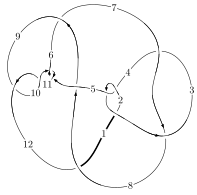
\includegraphics[width=112pt]{../../../GIT/diagram.site/Diagrams/png/2249_12n_0160.png}\\
\ \ \ A knot diagram\footnotemark}&
\allowdisplaybreaks
\textbf{Linearized knot diagam} \\
\cline{2-2}
 &
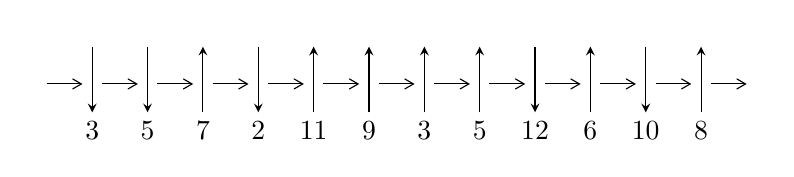
\begin{tikzpicture}[x=20pt, y=17pt]
	% nodes
	\node (C0) at (0, 0) {};
	\node (C1) at (1, 0) {};
	\node (C1U) at (1, +1) {};
	\node (C1D) at (1, -1) {3};

	\node (C2) at (2, 0) {};
	\node (C2U) at (2, +1) {};
	\node (C2D) at (2, -1) {5};

	\node (C3) at (3, 0) {};
	\node (C3U) at (3, +1) {};
	\node (C3D) at (3, -1) {7};

	\node (C4) at (4, 0) {};
	\node (C4U) at (4, +1) {};
	\node (C4D) at (4, -1) {2};

	\node (C5) at (5, 0) {};
	\node (C5U) at (5, +1) {};
	\node (C5D) at (5, -1) {11};

	\node (C6) at (6, 0) {};
	\node (C6U) at (6, +1) {};
	\node (C6D) at (6, -1) {9};

	\node (C7) at (7, 0) {};
	\node (C7U) at (7, +1) {};
	\node (C7D) at (7, -1) {3};

	\node (C8) at (8, 0) {};
	\node (C8U) at (8, +1) {};
	\node (C8D) at (8, -1) {5};

	\node (C9) at (9, 0) {};
	\node (C9U) at (9, +1) {};
	\node (C9D) at (9, -1) {12};

	\node (C10) at (10, 0) {};
	\node (C10U) at (10, +1) {};
	\node (C10D) at (10, -1) {6};

	\node (C11) at (11, 0) {};
	\node (C11U) at (11, +1) {};
	\node (C11D) at (11, -1) {10};

	\node (C12) at (12, 0) {};
	\node (C12U) at (12, +1) {};
	\node (C12D) at (12, -1) {8};
	\node (C13) at (13, 0) {};

	% arrows
	\draw[->,>={angle 60}]
	(C0) edge (C1) (C1) edge (C2) (C2) edge (C3) (C3) edge (C4) (C4) edge (C5) (C5) edge (C6) (C6) edge (C7) (C7) edge (C8) (C8) edge (C9) (C9) edge (C10) (C10) edge (C11) (C11) edge (C12) (C12) edge (C13) ;	\draw[->,>=stealth]
	(C1U) edge (C1D) (C2U) edge (C2D) (C3D) edge (C3U) (C4U) edge (C4D) (C5D) edge (C5U) (C6D) edge (C6U) (C7D) edge (C7U) (C8D) edge (C8U) (C9U) edge (C9D) (C10D) edge (C10U) (C11U) edge (C11D) (C12D) edge (C12U) ;
	\end{tikzpicture} \\
\hhline{~~} \\& 
\textbf{Solving Sequence} \\ \cline{2-2} 
 &
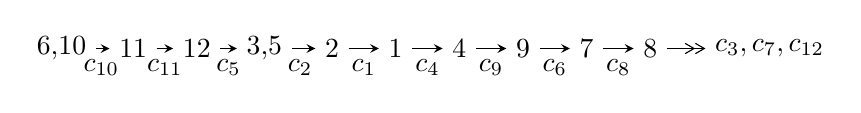
\begin{tikzpicture}[x=23pt, y=7pt]
	% node
	\node (A0) at (-1/8, 0) {6,10};
	\node (A1) at (1, 0) {11};
	\node (A2) at (2, 0) {12};
	\node (A3) at (49/16, 0) {3,5};
	\node (A4) at (33/8, 0) {2};
	\node (A5) at (41/8, 0) {1};
	\node (A6) at (49/8, 0) {4};
	\node (A7) at (57/8, 0) {9};
	\node (A8) at (65/8, 0) {7};
	\node (A9) at (73/8, 0) {8};
	\node (C1) at (1/2, -1) {$c_{10}$};
	\node (C2) at (3/2, -1) {$c_{11}$};
	\node (C3) at (5/2, -1) {$c_{5}$};
	\node (C4) at (29/8, -1) {$c_{2}$};
	\node (C5) at (37/8, -1) {$c_{1}$};
	\node (C6) at (45/8, -1) {$c_{4}$};
	\node (C7) at (53/8, -1) {$c_{9}$};
	\node (C8) at (61/8, -1) {$c_{6}$};
	\node (C9) at (69/8, -1) {$c_{8}$};
	\node (A10) at (11, 0) {$c_{3},c_{7},c_{12}$};

	% edge
	\draw[->,>=stealth]	
	(A0) edge (A1) (A1) edge (A2) (A2) edge (A3) (A3) edge (A4) (A4) edge (A5) (A5) edge (A6) (A6) edge (A7) (A7) edge (A8) (A8) edge (A9) ;
	\draw[->>,>={angle 60}]	
	(A9) edge (A10);
\end{tikzpicture} \\ 

\end{tabular} \\

\footnotetext{
The image of knot diagram is generated by the software ``\textbf{Draw programme}" developed by Andrew Bartholomew(\url{http://www.layer8.co.uk/maths/draw/index.htm\#Running-draw}), where we modified some parts for our purpose(\url{https://github.com/CATsTAILs/LinksPainter}).
}\phantom \\ \newline 
\centering \textbf{Ideals for irreducible components\footnotemark of $X_{\text{par}}$} 
 
\begin{align*}
I^u_{1}&=\langle 
-3 u^{34}+6 u^{33}+\cdots+b-3,\;3 u^{34}-3 u^{33}+\cdots+a+1,\;u^{35}-2 u^{34}+\cdots-2 u^2-1\rangle \\
I^u_{2}&=\langle 
- u^7- u^5-2 u^3+u^2+b- u,\;- u^6- u^4-2 u^2+a+u-1,\;u^9+u^8+2 u^7+u^6+3 u^5+u^4+2 u^3+u-1\rangle \\
\\
\end{align*}
\raggedright * 2 irreducible components of $\dim_{\mathbb{C}}=0$, with total 44 representations.\\
\footnotetext{All coefficients of polynomials are rational numbers. But the coefficients are sometimes approximated in decimal forms when there is not enough margin.}
\newpage
\renewcommand{\arraystretch}{1}
\centering \section*{I. $I^u_{1}= \langle -3 u^{34}+6 u^{33}+\cdots+b-3,\;3 u^{34}-3 u^{33}+\cdots+a+1,\;u^{35}-2 u^{34}+\cdots-2 u^2-1 \rangle$}
\flushleft \textbf{(i) Arc colorings}\\
\begin{tabular}{m{7pt} m{180pt} m{7pt} m{180pt} }
\flushright $a_{6}=$&$\begin{pmatrix}0\\u\end{pmatrix}$ \\
\flushright $a_{10}=$&$\begin{pmatrix}1\\0\end{pmatrix}$ \\
\flushright $a_{11}=$&$\begin{pmatrix}1\\- u^2\end{pmatrix}$ \\
\flushright $a_{12}=$&$\begin{pmatrix}u^2+1\\- u^2\end{pmatrix}$ \\
\flushright $a_{3}=$&$\begin{pmatrix}-3 u^{34}+3 u^{33}+\cdots-2 u-1\\3 u^{34}-6 u^{33}+\cdots+u+3\end{pmatrix}$ \\
\flushright $a_{5}=$&$\begin{pmatrix}- u\\u^3+u\end{pmatrix}$ \\
\flushright $a_{2}=$&$\begin{pmatrix}-2 u^{34}+2 u^{33}+\cdots-2 u-1\\2 u^{34}-4 u^{33}+\cdots+7 u^2+2\end{pmatrix}$ \\
\flushright $a_{1}=$&$\begin{pmatrix}- u^{20}-3 u^{18}-7 u^{16}-10 u^{14}-10 u^{12}-7 u^{10}- u^8+2 u^6+3 u^4+u^2-1\\u^{22}+4 u^{20}+\cdots+2 u^4+u^2\end{pmatrix}$ \\
\flushright $a_{4}=$&$\begin{pmatrix}- u^{34}+u^{33}+\cdots+3 u^2-3 u\\u^{34}-2 u^{33}+\cdots+4 u^2+1\end{pmatrix}$ \\
\flushright $a_{9}=$&$\begin{pmatrix}u^4+u^2+1\\- u^4\end{pmatrix}$ \\
\flushright $a_{7}=$&$\begin{pmatrix}u^9+2 u^7+3 u^5+2 u^3+u\\- u^9- u^7- u^5+u\end{pmatrix}$ \\
\flushright $a_{8}=$&$\begin{pmatrix}- u^8- u^6- u^4+1\\u^{10}+2 u^8+3 u^6+2 u^4+u^2\end{pmatrix}$\\&\end{tabular}
\flushleft \textbf{(ii) Obstruction class $= -1$}\\~\\
\flushleft \textbf{(iii) Cusp Shapes $= 4 u^{34}-2 u^{33}+24 u^{32}-8 u^{31}+92 u^{30}-18 u^{29}+247 u^{28}-13 u^{27}+523 u^{26}+50 u^{25}+904 u^{24}+221 u^{23}+1321 u^{22}+524 u^{21}+1669 u^{20}+895 u^{19}+1845 u^{18}+1222 u^{17}+1810 u^{16}+1360 u^{15}+1576 u^{14}+1256 u^{13}+1216 u^{12}+958 u^{11}+820 u^{10}+594 u^9+460 u^8+299 u^7+205 u^6+110 u^5+63 u^4+27 u^3+5 u^2+4 u-2$}\\~\\
\newpage\renewcommand{\arraystretch}{1}
\flushleft \textbf{(iv) u-Polynomials at the component}\newline \\
\begin{tabular}{m{50pt}|m{274pt}}
Crossings & \hspace{64pt}u-Polynomials at each crossing \\
\hline $$\begin{aligned}c_{1}\end{aligned}$$&$\begin{aligned}
&u^{35}+52 u^{34}+\cdots+32 u+1
\end{aligned}$\\
\hline $$\begin{aligned}c_{2},c_{4}\end{aligned}$$&$\begin{aligned}
&u^{35}-10 u^{34}+\cdots+12 u-1
\end{aligned}$\\
\hline $$\begin{aligned}c_{3},c_{7}\end{aligned}$$&$\begin{aligned}
&u^{35}- u^{34}+\cdots-1024 u-512
\end{aligned}$\\
\hline $$\begin{aligned}c_{5},c_{10}\end{aligned}$$&$\begin{aligned}
&u^{35}-2 u^{34}+\cdots-2 u^2-1
\end{aligned}$\\
\hline $$\begin{aligned}c_{6}\end{aligned}$$&$\begin{aligned}
&u^{35}+10 u^{34}+\cdots-206 u-31
\end{aligned}$\\
\hline $$\begin{aligned}c_{8}\end{aligned}$$&$\begin{aligned}
&u^{35}-2 u^{34}+\cdots-412 u-241
\end{aligned}$\\
\hline $$\begin{aligned}c_{9},c_{11}\end{aligned}$$&$\begin{aligned}
&u^{35}+12 u^{34}+\cdots-4 u-1
\end{aligned}$\\
\hline $$\begin{aligned}c_{12}\end{aligned}$$&$\begin{aligned}
&u^{35}+36 u^{33}+\cdots-2 u-1
\end{aligned}$\\
\hline
\end{tabular}\\~\\
\newpage\renewcommand{\arraystretch}{1}
\flushleft \textbf{(v) Riley Polynomials at the component}\newline \\
\begin{tabular}{m{50pt}|m{274pt}}
Crossings & \hspace{64pt}Riley Polynomials at each crossing \\
\hline $$\begin{aligned}c_{1}\end{aligned}$$&$\begin{aligned}
&y^{35}-128 y^{34}+\cdots+420 y-1
\end{aligned}$\\
\hline $$\begin{aligned}c_{2},c_{4}\end{aligned}$$&$\begin{aligned}
&y^{35}-52 y^{34}+\cdots+32 y-1
\end{aligned}$\\
\hline $$\begin{aligned}c_{3},c_{7}\end{aligned}$$&$\begin{aligned}
&y^{35}+57 y^{34}+\cdots+2621440 y-262144
\end{aligned}$\\
\hline $$\begin{aligned}c_{5},c_{10}\end{aligned}$$&$\begin{aligned}
&y^{35}+12 y^{34}+\cdots-4 y-1
\end{aligned}$\\
\hline $$\begin{aligned}c_{6}\end{aligned}$$&$\begin{aligned}
&y^{35}+12 y^{34}+\cdots-10140 y-961
\end{aligned}$\\
\hline $$\begin{aligned}c_{8}\end{aligned}$$&$\begin{aligned}
&y^{35}+12 y^{34}+\cdots-1095024 y-58081
\end{aligned}$\\
\hline $$\begin{aligned}c_{9},c_{11}\end{aligned}$$&$\begin{aligned}
&y^{35}+24 y^{34}+\cdots-16 y-1
\end{aligned}$\\
\hline $$\begin{aligned}c_{12}\end{aligned}$$&$\begin{aligned}
&y^{35}+72 y^{34}+\cdots-4 y-1
\end{aligned}$\\
\hline
\end{tabular}\\~\\
\newpage\flushleft \textbf{(vi) Complex Volumes and Cusp Shapes}
$$\begin{array}{c|c|c}  
\text{Solutions to }I^u_{1}& \I (\text{vol} + \sqrt{-1}CS) & \text{Cusp shape}\\
 \hline 
\begin{aligned}
u &= \phantom{-}0.737220 + 0.648144 I \\
a &= \phantom{-}1.74315 - 1.73886 I \\
b &= -2.41211 + 0.15211 I\end{aligned}
 & -0.58521 - 2.05799 I & \phantom{-}0.94554 + 1.75994 I \\ \hline\begin{aligned}
u &= \phantom{-}0.737220 - 0.648144 I \\
a &= \phantom{-}1.74315 + 1.73886 I \\
b &= -2.41211 - 0.15211 I\end{aligned}
 & -0.58521 + 2.05799 I & \phantom{-}0.94554 - 1.75994 I \\ \hline\begin{aligned}
u &= \phantom{-}0.101201 + 0.967150 I \\
a &= -0.223398 - 0.378771 I \\
b &= -0.343721 + 0.254391 I\end{aligned}
 & -2.08113 + 1.70930 I & \phantom{-}0.77222 - 3.96512 I \\ \hline\begin{aligned}
u &= \phantom{-}0.101201 - 0.967150 I \\
a &= -0.223398 + 0.378771 I \\
b &= -0.343721 - 0.254391 I\end{aligned}
 & -2.08113 - 1.70930 I & \phantom{-}0.77222 + 3.96512 I \\ \hline\begin{aligned}
u &= \phantom{-}0.678017 + 0.796351 I \\
a &= -1.63124 - 0.26748 I \\
b &= \phantom{-}0.89300 + 1.48039 I\end{aligned}
 & \phantom{-}1.40101 + 2.20417 I & \phantom{-}3.92249 - 4.39905 I \\ \hline\begin{aligned}
u &= \phantom{-}0.678017 - 0.796351 I \\
a &= -1.63124 + 0.26748 I \\
b &= \phantom{-}0.89300 - 1.48039 I\end{aligned}
 & \phantom{-}1.40101 - 2.20417 I & \phantom{-}3.92249 + 4.39905 I \\ \hline\begin{aligned}
u &= -0.030827 + 1.048300 I \\
a &= \phantom{-}0.987634 + 0.536168 I \\
b &= \phantom{-}0.592511 - 1.018810 I\end{aligned}
 & -6.06605 - 1.60204 I & -6.58193 + 1.49646 I \\ \hline\begin{aligned}
u &= -0.030827 - 1.048300 I \\
a &= \phantom{-}0.987634 - 0.536168 I \\
b &= \phantom{-}0.592511 + 1.018810 I\end{aligned}
 & -6.06605 + 1.60204 I & -6.58193 - 1.49646 I \\ \hline\begin{aligned}
u &= \phantom{-}0.838636 + 0.644982 I \\
a &= -0.76138 + 2.67985 I \\
b &= \phantom{-}2.36698 - 1.75635 I\end{aligned}
 & -10.48130 - 6.27093 I & \phantom{-}0.94475 + 1.94965 I \\ \hline\begin{aligned}
u &= \phantom{-}0.838636 - 0.644982 I \\
a &= -0.76138 - 2.67985 I \\
b &= \phantom{-}2.36698 + 1.75635 I\end{aligned}
 & -10.48130 + 6.27093 I & \phantom{-}0.94475 - 1.94965 I\\
 \hline 
 \end{array}$$\newpage$$\begin{array}{c|c|c}  
\text{Solutions to }I^u_{1}& \I (\text{vol} + \sqrt{-1}CS) & \text{Cusp shape}\\
 \hline 
\begin{aligned}
u &= -0.781183 + 0.727089 I \\
a &= -0.051887 + 0.135238 I \\
b &= \phantom{-}0.057797 + 0.143372 I\end{aligned}
 & \phantom{-}3.78767 + 1.08265 I & \phantom{-}9.73080 - 0.41634 I \\ \hline\begin{aligned}
u &= -0.781183 - 0.727089 I \\
a &= -0.051887 - 0.135238 I \\
b &= \phantom{-}0.057797 - 0.143372 I\end{aligned}
 & \phantom{-}3.78767 - 1.08265 I & \phantom{-}9.73080 + 0.41634 I \\ \hline\begin{aligned}
u &= -0.632282 + 0.665654 I \\
a &= \phantom{-}0.152240 - 0.624708 I \\
b &= -0.319580 - 0.496331 I\end{aligned}
 & -1.37778 - 0.83460 I & \phantom{-}0.396623 + 0.019030 I \\ \hline\begin{aligned}
u &= -0.632282 - 0.665654 I \\
a &= \phantom{-}0.152240 + 0.624708 I \\
b &= -0.319580 + 0.496331 I\end{aligned}
 & -1.37778 + 0.83460 I & \phantom{-}0.396623 - 0.019030 I \\ \hline\begin{aligned}
u &= -0.121893 + 1.112050 I \\
a &= -1.224660 - 0.088950 I \\
b &= -0.248194 + 1.351040 I\end{aligned}
 & -17.1086 - 5.6948 I & -5.50780 + 3.28741 I \\ \hline\begin{aligned}
u &= -0.121893 - 1.112050 I \\
a &= -1.224660 + 0.088950 I \\
b &= -0.248194 - 1.351040 I\end{aligned}
 & -17.1086 + 5.6948 I & -5.50780 - 3.28741 I \\ \hline\begin{aligned}
u &= \phantom{-}0.660177 + 0.922712 I \\
a &= \phantom{-}0.183127 - 1.365060 I \\
b &= -1.38045 + 0.73221 I\end{aligned}
 & \phantom{-}1.00684 + 2.97409 I & \phantom{-}3.31167 - 1.92596 I \\ \hline\begin{aligned}
u &= \phantom{-}0.660177 - 0.922712 I \\
a &= \phantom{-}0.183127 + 1.365060 I \\
b &= -1.38045 - 0.73221 I\end{aligned}
 & \phantom{-}1.00684 - 2.97409 I & \phantom{-}3.31167 + 1.92596 I \\ \hline\begin{aligned}
u &= -0.518083 + 1.034140 I \\
a &= -0.493003 + 0.558538 I \\
b &= \phantom{-}0.322191 + 0.799204 I\end{aligned}
 & -14.7020 - 1.1608 I & -3.27320 + 2.65041 I \\ \hline\begin{aligned}
u &= -0.518083 - 1.034140 I \\
a &= -0.493003 - 0.558538 I \\
b &= \phantom{-}0.322191 - 0.799204 I\end{aligned}
 & -14.7020 + 1.1608 I & -3.27320 - 2.65041 I\\
 \hline 
 \end{array}$$\newpage$$\begin{array}{c|c|c}  
\text{Solutions to }I^u_{1}& \I (\text{vol} + \sqrt{-1}CS) & \text{Cusp shape}\\
 \hline 
\begin{aligned}
u &= -0.645286 + 0.989574 I \\
a &= \phantom{-}0.110285 - 0.455498 I \\
b &= -0.379583 - 0.403061 I\end{aligned}
 & -2.35824 - 4.23049 I & -1.64611 + 4.83730 I \\ \hline\begin{aligned}
u &= -0.645286 - 0.989574 I \\
a &= \phantom{-}0.110285 + 0.455498 I \\
b &= -0.379583 + 0.403061 I\end{aligned}
 & -2.35824 + 4.23049 I & -1.64611 - 4.83730 I \\ \hline\begin{aligned}
u &= \phantom{-}0.801511 + 0.879701 I \\
a &= \phantom{-}1.77931 + 2.04057 I \\
b &= \phantom{-}0.36896 - 3.20080 I\end{aligned}
 & -6.25391 + 2.99402 I & \phantom{-}1.83860 - 2.69092 I \\ \hline\begin{aligned}
u &= \phantom{-}0.801511 - 0.879701 I \\
a &= \phantom{-}1.77931 - 2.04057 I \\
b &= \phantom{-}0.36896 + 3.20080 I\end{aligned}
 & -6.25391 - 2.99402 I & \phantom{-}1.83860 + 2.69092 I \\ \hline\begin{aligned}
u &= \phantom{-}0.677300 + 1.008060 I \\
a &= -2.02100 + 1.40176 I \\
b &= \phantom{-}2.78188 + 1.08787 I\end{aligned}
 & -1.65574 + 7.47330 I & -0.96819 - 6.53783 I \\ \hline\begin{aligned}
u &= \phantom{-}0.677300 - 1.008060 I \\
a &= -2.02100 - 1.40176 I \\
b &= \phantom{-}2.78188 - 1.08787 I\end{aligned}
 & -1.65574 - 7.47330 I & -0.96819 + 6.53783 I \\ \hline\begin{aligned}
u &= -0.718651 + 0.985154 I \\
a &= \phantom{-}0.0048122 + 0.1319630 I \\
b &= \phantom{-}0.133462 + 0.090095 I\end{aligned}
 & \phantom{-}3.00104 - 6.75637 I & \phantom{-}7.73187 + 5.52332 I \\ \hline\begin{aligned}
u &= -0.718651 - 0.985154 I \\
a &= \phantom{-}0.0048122 - 0.1319630 I \\
b &= \phantom{-}0.133462 - 0.090095 I\end{aligned}
 & \phantom{-}3.00104 + 6.75637 I & \phantom{-}7.73187 - 5.52332 I \\ \hline\begin{aligned}
u &= -0.715979 + 0.271293 I \\
a &= \phantom{-}0.797619 + 0.724413 I \\
b &= \phantom{-}0.767607 + 0.302276 I\end{aligned}
 & -12.50660 - 3.28011 I & \phantom{-}0.69781 + 2.19401 I \\ \hline\begin{aligned}
u &= -0.715979 - 0.271293 I \\
a &= \phantom{-}0.797619 - 0.724413 I \\
b &= \phantom{-}0.767607 - 0.302276 I\end{aligned}
 & -12.50660 + 3.28011 I & \phantom{-}0.69781 - 2.19401 I\\
 \hline 
 \end{array}$$\newpage$$\begin{array}{c|c|c}  
\text{Solutions to }I^u_{1}& \I (\text{vol} + \sqrt{-1}CS) & \text{Cusp shape}\\
 \hline 
\begin{aligned}
u &= \phantom{-}0.715761 + 1.041330 I \\
a &= \phantom{-}2.74535 - 0.31064 I \\
b &= -2.28849 - 2.63647 I\end{aligned}
 & -11.6867 + 12.0828 I & -0.83819 - 6.56234 I \\ \hline\begin{aligned}
u &= \phantom{-}0.715761 - 1.041330 I \\
a &= \phantom{-}2.74535 + 0.31064 I \\
b &= -2.28849 + 2.63647 I\end{aligned}
 & -11.6867 - 12.0828 I & -0.83819 + 6.56234 I \\ \hline\begin{aligned}
u &= -0.268541 + 0.381611 I \\
a &= \phantom{-}0.20602 - 1.57922 I \\
b &= -0.547327 - 0.502704 I\end{aligned}
 & -1.72551 - 0.80413 I & -2.43242 + 1.76310 I \\ \hline\begin{aligned}
u &= -0.268541 - 0.381611 I \\
a &= \phantom{-}0.20602 + 1.57922 I \\
b &= -0.547327 + 0.502704 I\end{aligned}
 & -1.72551 + 0.80413 I & -2.43242 - 1.76310 I \\ \hline\begin{aligned}
u &= \phantom{-}0.445806\phantom{ +0.000000I} \\
a &= -0.605941\phantom{ +0.000000I} \\
b &= \phantom{-}0.270132\phantom{ +0.000000I}\end{aligned}
 & \phantom{-}0.870658\phantom{ +0.000000I} & \phantom{-}11.9110\phantom{ +0.000000I}\\
 \hline 
 \end{array}$$\newpage\newpage\renewcommand{\arraystretch}{1}
\centering \section*{II. $I^u_{2}= \langle - u^7- u^5-2 u^3+u^2+b- u,\;- u^6- u^4-2 u^2+a+u-1,\;u^9+u^8+2 u^7+u^6+3 u^5+u^4+2 u^3+u-1 \rangle$}
\flushleft \textbf{(i) Arc colorings}\\
\begin{tabular}{m{7pt} m{180pt} m{7pt} m{180pt} }
\flushright $a_{6}=$&$\begin{pmatrix}0\\u\end{pmatrix}$ \\
\flushright $a_{10}=$&$\begin{pmatrix}1\\0\end{pmatrix}$ \\
\flushright $a_{11}=$&$\begin{pmatrix}1\\- u^2\end{pmatrix}$ \\
\flushright $a_{12}=$&$\begin{pmatrix}u^2+1\\- u^2\end{pmatrix}$ \\
\flushright $a_{3}=$&$\begin{pmatrix}u^6+u^4+2 u^2- u+1\\u^7+u^5+2 u^3- u^2+u\end{pmatrix}$ \\
\flushright $a_{5}=$&$\begin{pmatrix}- u\\u^3+u\end{pmatrix}$ \\
\flushright $a_{2}=$&$\begin{pmatrix}u^6+u^4+2 u^2+1\\u^7+u^5+u^3- u^2\end{pmatrix}$ \\
\flushright $a_{1}=$&$\begin{pmatrix}u\\- u^3- u\end{pmatrix}$ \\
\flushright $a_{4}=$&$\begin{pmatrix}u^6+u^4+2 u^2- u+1\\u^7+u^5+2 u^3- u^2+u\end{pmatrix}$ \\
\flushright $a_{9}=$&$\begin{pmatrix}u^4+u^2+1\\- u^4\end{pmatrix}$ \\
\flushright $a_{7}=$&$\begin{pmatrix}- u^8- u^6- u^4+1\\u^8+u^7+u^6+2 u^5+u^4+2 u^3+2 u-1\end{pmatrix}$ \\
\flushright $a_{8}=$&$\begin{pmatrix}- u^8- u^6- u^4+1\\u^8+u^7+u^6+2 u^5+u^4+2 u^3+2 u-1\end{pmatrix}$\\&\end{tabular}
\flushleft \textbf{(ii) Obstruction class $= 1$}\\~\\
\flushleft \textbf{(iii) Cusp Shapes $= 4 u^7+4 u^6+3 u^5+3 u^4+6 u^3+3 u^2- u+1$}\\~\\
\newpage\renewcommand{\arraystretch}{1}
\flushleft \textbf{(iv) u-Polynomials at the component}\newline \\
\begin{tabular}{m{50pt}|m{274pt}}
Crossings & \hspace{64pt}u-Polynomials at each crossing \\
\hline $$\begin{aligned}c_{1},c_{2}\end{aligned}$$&$\begin{aligned}
&(u-1)^9
\end{aligned}$\\
\hline $$\begin{aligned}c_{3},c_{7}\end{aligned}$$&$\begin{aligned}
&u^9
\end{aligned}$\\
\hline $$\begin{aligned}c_{4}\end{aligned}$$&$\begin{aligned}
&(u+1)^9
\end{aligned}$\\
\hline $$\begin{aligned}c_{5}\end{aligned}$$&$\begin{aligned}
&u^9- u^8+2 u^7- u^6+3 u^5- u^4+2 u^3+u+1
\end{aligned}$\\
\hline $$\begin{aligned}c_{6}\end{aligned}$$&$\begin{aligned}
&u^9+5 u^8+12 u^7+15 u^6+9 u^5- u^4-4 u^3-2 u^2+u+1
\end{aligned}$\\
\hline $$\begin{aligned}c_{8},c_{12}\end{aligned}$$&$\begin{aligned}
&u^9+u^8-2 u^7-3 u^6+u^5+3 u^4+2 u^3- u-1
\end{aligned}$\\
\hline $$\begin{aligned}c_{9}\end{aligned}$$&$\begin{aligned}
&u^9-3 u^8+8 u^7-13 u^6+17 u^5-17 u^4+12 u^3-6 u^2+u+1
\end{aligned}$\\
\hline $$\begin{aligned}c_{10}\end{aligned}$$&$\begin{aligned}
&u^9+u^8+2 u^7+u^6+3 u^5+u^4+2 u^3+u-1
\end{aligned}$\\
\hline $$\begin{aligned}c_{11}\end{aligned}$$&$\begin{aligned}
&u^9+3 u^8+8 u^7+13 u^6+17 u^5+17 u^4+12 u^3+6 u^2+u-1
\end{aligned}$\\
\hline
\end{tabular}\\~\\
\newpage\renewcommand{\arraystretch}{1}
\flushleft \textbf{(v) Riley Polynomials at the component}\newline \\
\begin{tabular}{m{50pt}|m{274pt}}
Crossings & \hspace{64pt}Riley Polynomials at each crossing \\
\hline $$\begin{aligned}c_{1},c_{2},c_{4}\end{aligned}$$&$\begin{aligned}
&(y-1)^9
\end{aligned}$\\
\hline $$\begin{aligned}c_{3},c_{7}\end{aligned}$$&$\begin{aligned}
&y^9
\end{aligned}$\\
\hline $$\begin{aligned}c_{5},c_{10}\end{aligned}$$&$\begin{aligned}
&y^9+3 y^8+8 y^7+13 y^6+17 y^5+17 y^4+12 y^3+6 y^2+y-1
\end{aligned}$\\
\hline $$\begin{aligned}c_{6}\end{aligned}$$&$\begin{aligned}
&y^9- y^8+12 y^7-7 y^6+37 y^5+y^4-10 y^2+5 y-1
\end{aligned}$\\
\hline $$\begin{aligned}c_{8},c_{12}\end{aligned}$$&$\begin{aligned}
&y^9-5 y^8+12 y^7-15 y^6+9 y^5+y^4-4 y^3+2 y^2+y-1
\end{aligned}$\\
\hline $$\begin{aligned}c_{9},c_{11}\end{aligned}$$&$\begin{aligned}
&y^9+7 y^8+20 y^7+25 y^6+5 y^5-15 y^4+22 y^2+13 y-1
\end{aligned}$\\
\hline
\end{tabular}\\~\\
\newpage\flushleft \textbf{(vi) Complex Volumes and Cusp Shapes}
$$\begin{array}{c|c|c}  
\text{Solutions to }I^u_{2}& \I (\text{vol} + \sqrt{-1}CS) & \text{Cusp shape}\\
 \hline 
\begin{aligned}
u &= \phantom{-}0.140343 + 0.966856 I \\
a &= -0.770941 - 0.258974 I \\
b &= \phantom{-}0.142194 - 0.781734 I\end{aligned}
 & -3.42837 + 2.09337 I & -5.30979 - 3.87975 I \\ \hline\begin{aligned}
u &= \phantom{-}0.140343 - 0.966856 I \\
a &= -0.770941 + 0.258974 I \\
b &= \phantom{-}0.142194 + 0.781734 I\end{aligned}
 & -3.42837 - 2.09337 I & -5.30979 + 3.87975 I \\ \hline\begin{aligned}
u &= \phantom{-}0.628449 + 0.875112 I \\
a &= -0.147409 - 0.367985 I \\
b &= \phantom{-}0.229389 - 0.360259 I\end{aligned}
 & -1.02799 + 2.45442 I & \phantom{-}0.49381 - 3.35442 I \\ \hline\begin{aligned}
u &= \phantom{-}0.628449 - 0.875112 I \\
a &= -0.147409 + 0.367985 I \\
b &= \phantom{-}0.229389 + 0.360259 I\end{aligned}
 & -1.02799 - 2.45442 I & \phantom{-}0.49381 + 3.35442 I \\ \hline\begin{aligned}
u &= -0.796005 + 0.733148 I \\
a &= \phantom{-}0.24323 - 1.73417 I \\
b &= \phantom{-}1.07779 + 1.55873 I\end{aligned}
 & \phantom{-}2.72642 + 1.33617 I & \phantom{-}1.53709 - 1.22905 I \\ \hline\begin{aligned}
u &= -0.796005 - 0.733148 I \\
a &= \phantom{-}0.24323 + 1.73417 I \\
b &= \phantom{-}1.07779 - 1.55873 I\end{aligned}
 & \phantom{-}2.72642 - 1.33617 I & \phantom{-}1.53709 + 1.22905 I \\ \hline\begin{aligned}
u &= -0.728966 + 0.986295 I \\
a &= \phantom{-}1.62529 - 0.46000 I \\
b &= -0.73109 + 1.93833 I\end{aligned}
 & \phantom{-}1.95319 - 7.08493 I & \phantom{-}0.02676 + 6.64241 I \\ \hline\begin{aligned}
u &= -0.728966 - 0.986295 I \\
a &= \phantom{-}1.62529 + 0.46000 I \\
b &= -0.73109 - 1.93833 I\end{aligned}
 & \phantom{-}1.95319 + 7.08493 I & \phantom{-}0.02676 - 6.64241 I \\ \hline\begin{aligned}
u &= \phantom{-}0.512358\phantom{ +0.000000I} \\
a &= \phantom{-}1.09967\phantom{ +0.000000I} \\
b &= \phantom{-}0.563422\phantom{ +0.000000I}\end{aligned}
 & -0.446489\phantom{ +0.000000I} & \phantom{-}2.50430\phantom{ +0.000000I}\\
 \hline 
 \end{array}$$\newpage
\newpage\renewcommand{\arraystretch}{1}
\centering \section*{ III. u-Polynomials}
\begin{tabular}{m{50pt}|m{274pt}}
Crossings & \hspace{64pt}u-Polynomials at each crossing \\
\hline $$\begin{aligned}c_{1}\end{aligned}$$&$\begin{aligned}
&((u-1)^9)(u^{35}+52 u^{34}+\cdots+32 u+1)
\end{aligned}$\\
\hline $$\begin{aligned}c_{2}\end{aligned}$$&$\begin{aligned}
&((u-1)^9)(u^{35}-10 u^{34}+\cdots+12 u-1)
\end{aligned}$\\
\hline $$\begin{aligned}c_{3},c_{7}\end{aligned}$$&$\begin{aligned}
&u^9(u^{35}- u^{34}+\cdots-1024 u-512)
\end{aligned}$\\
\hline $$\begin{aligned}c_{4}\end{aligned}$$&$\begin{aligned}
&((u+1)^9)(u^{35}-10 u^{34}+\cdots+12 u-1)
\end{aligned}$\\
\hline $$\begin{aligned}c_{5}\end{aligned}$$&$\begin{aligned}
&(u^9- u^8+\cdots+u+1)(u^{35}-2 u^{34}+\cdots-2 u^2-1)
\end{aligned}$\\
\hline $$\begin{aligned}c_{6}\end{aligned}$$&$\begin{aligned}
&(u^9+5 u^8+12 u^7+15 u^6+9 u^5- u^4-4 u^3-2 u^2+u+1)\\
&\cdot(u^{35}+10 u^{34}+\cdots-206 u-31)
\end{aligned}$\\
\hline $$\begin{aligned}c_{8}\end{aligned}$$&$\begin{aligned}
&(u^9+u^8-2 u^7-3 u^6+u^5+3 u^4+2 u^3- u-1)\\
&\cdot(u^{35}-2 u^{34}+\cdots-412 u-241)
\end{aligned}$\\
\hline $$\begin{aligned}c_{9}\end{aligned}$$&$\begin{aligned}
&(u^9-3 u^8+8 u^7-13 u^6+17 u^5-17 u^4+12 u^3-6 u^2+u+1)\\
&\cdot(u^{35}+12 u^{34}+\cdots-4 u-1)
\end{aligned}$\\
\hline $$\begin{aligned}c_{10}\end{aligned}$$&$\begin{aligned}
&(u^9+u^8+\cdots+u-1)(u^{35}-2 u^{34}+\cdots-2 u^2-1)
\end{aligned}$\\
\hline $$\begin{aligned}c_{11}\end{aligned}$$&$\begin{aligned}
&(u^9+3 u^8+8 u^7+13 u^6+17 u^5+17 u^4+12 u^3+6 u^2+u-1)\\
&\cdot(u^{35}+12 u^{34}+\cdots-4 u-1)
\end{aligned}$\\
\hline $$\begin{aligned}c_{12}\end{aligned}$$&$\begin{aligned}
&(u^9+u^8-2 u^7-3 u^6+u^5+3 u^4+2 u^3- u-1)\\
&\cdot(u^{35}+36 u^{33}+\cdots-2 u-1)
\end{aligned}$\\
\hline
\end{tabular}\newpage\renewcommand{\arraystretch}{1}
\centering \section*{ IV. Riley Polynomials}
\begin{tabular}{m{50pt}|m{274pt}}
Crossings & \hspace{64pt}Riley Polynomials at each crossing \\
\hline $$\begin{aligned}c_{1}\end{aligned}$$&$\begin{aligned}
&((y-1)^9)(y^{35}-128 y^{34}+\cdots+420 y-1)
\end{aligned}$\\
\hline $$\begin{aligned}c_{2},c_{4}\end{aligned}$$&$\begin{aligned}
&((y-1)^9)(y^{35}-52 y^{34}+\cdots+32 y-1)
\end{aligned}$\\
\hline $$\begin{aligned}c_{3},c_{7}\end{aligned}$$&$\begin{aligned}
&y^9(y^{35}+57 y^{34}+\cdots+2621440 y-262144)
\end{aligned}$\\
\hline $$\begin{aligned}c_{5},c_{10}\end{aligned}$$&$\begin{aligned}
&(y^9+3 y^8+8 y^7+13 y^6+17 y^5+17 y^4+12 y^3+6 y^2+y-1)\\
&\cdot(y^{35}+12 y^{34}+\cdots-4 y-1)
\end{aligned}$\\
\hline $$\begin{aligned}c_{6}\end{aligned}$$&$\begin{aligned}
&(y^9- y^8+12 y^7-7 y^6+37 y^5+y^4-10 y^2+5 y-1)\\
&\cdot(y^{35}+12 y^{34}+\cdots-10140 y-961)
\end{aligned}$\\
\hline $$\begin{aligned}c_{8}\end{aligned}$$&$\begin{aligned}
&(y^9-5 y^8+12 y^7-15 y^6+9 y^5+y^4-4 y^3+2 y^2+y-1)\\
&\cdot(y^{35}+12 y^{34}+\cdots-1095024 y-58081)
\end{aligned}$\\
\hline $$\begin{aligned}c_{9},c_{11}\end{aligned}$$&$\begin{aligned}
&(y^9+7 y^8+20 y^7+25 y^6+5 y^5-15 y^4+22 y^2+13 y-1)\\
&\cdot(y^{35}+24 y^{34}+\cdots-16 y-1)
\end{aligned}$\\
\hline $$\begin{aligned}c_{12}\end{aligned}$$&$\begin{aligned}
&(y^9-5 y^8+12 y^7-15 y^6+9 y^5+y^4-4 y^3+2 y^2+y-1)\\
&\cdot(y^{35}+72 y^{34}+\cdots-4 y-1)
\end{aligned}$\\
\hline
\end{tabular}
\vskip 2pc
\end{document}